\documentclass[11pt]{amsart}
\usepackage{geometry}                % See geometry.pdf to learn the layout options. There are lots.
\geometry{letterpaper}                   % ... or a4paper or a5paper or ... 
\usepackage{graphicx}
\usepackage{amssymb}
\usepackage{epstopdf}
\DeclareGraphicsRule{.tif}{png}{.png}{`convert #1 `dirname #1`/`basename #1 .tif`.png}

\title{Final Report}
\author{Juan Durazo \\ Arthur Mitrano \\ Brendan Horan}
%\date{}                                           % Activate to display a given date or no date

\begin{document}
\maketitle
\section{ introduction}
\subsection{Problem} \indent \\
The problem we are seeking to solve is 
$$Ax=b, \indent A  \in  \mathbb{R}, \indent b = b^{exact} + b^{noise}$$ \\
In the above equation, $b^{noise}$ is a white noise vector with unknown level $\delta_{noise}$.
We investigate how noise enters the problem through $b$ and how it propagates into the 
core problem. Using this information, we can develop a stopping criteria for hybrid methods 
that are based on the Golub-Kahan bidiagonalization(GKb) process. Additionally, we 
can estimate the original noise level that was introduced into the problem with $b$.

\section{Cumulative Periododogram}
The Cumulative Periodogram(NCP) can be used to determine how "white-noise like" 
each $s_k$ is. Given a sequence of $s_k$ we can compute the vectors
$$c_k = |dft(s_k)|^2, \indent z_k = \frac{\sum_{i=1}^k c_i}{ \sum_{i=1}^q c_i}, \indent j=1,\cdots, q$$ 
The test is to see if any of the $z_k$ vectors are to a straight increasing diagonal line. There are two 
way to measure how close the $z_k$ vectors are to this diagonal line. We can measure the 
absolute value of the deviation of each vector from the "white noise" diagonal line or we can keep
count of the number of indices that lie outside the Kolmogorov-Smirnov test at a certain confidence 
level. We will consider several values for this confidence level in the results section.

\section{Results}

\subsection{Finding $\bf k_{noise}$ using GKB}
	Recall that we can find the iteration $k_{noise}$ in which the noise is revealed automatically
	using the noise-signal space computations and also by looking at plots of the $s_k$ vectors.
	For the purposes of discussion and demonstration, we will use the latter approach to present
	the results here.

	We first consider the case when $\delta_{noise}=10^{-14}$ and then consider the cases
	where $\delta_{noise} = 10^{-8},10^{-4},10^{-2}$:


	%%%%%%%%%%%%%%%%%%%%%%%%%%%%%%%%%%%%%%%%%%%%%%
	\vspace{5mm}
	\begin{minipage}[t]{0.5\textwidth}
	
		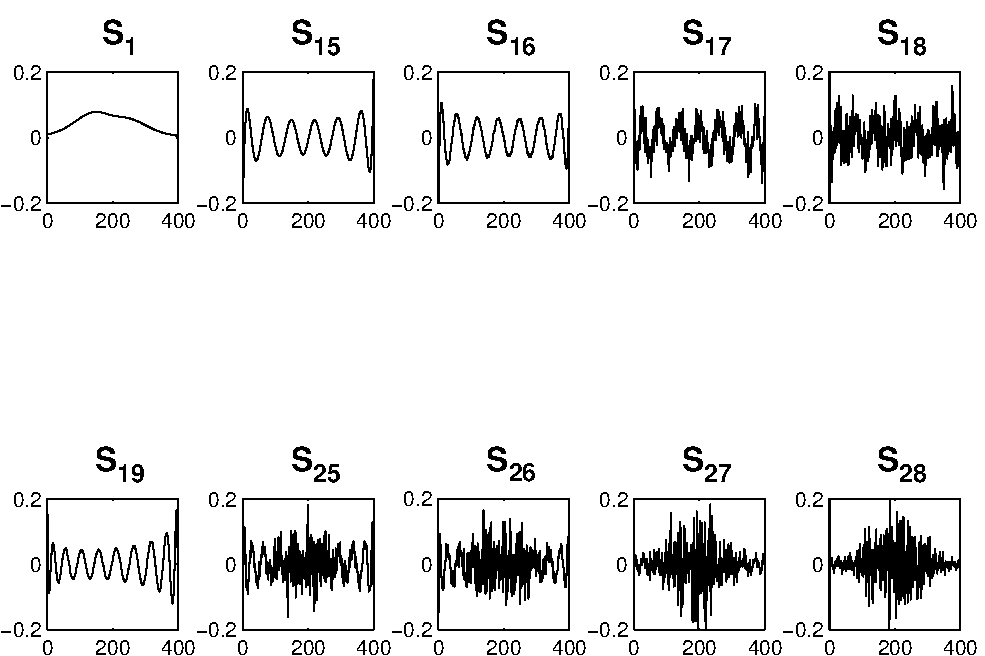
\includegraphics[width=.95\linewidth]{figures/run1/sk_plots} 
   
	\end{minipage}
	\begin{minipage}[t]{0.5\textwidth}
	
		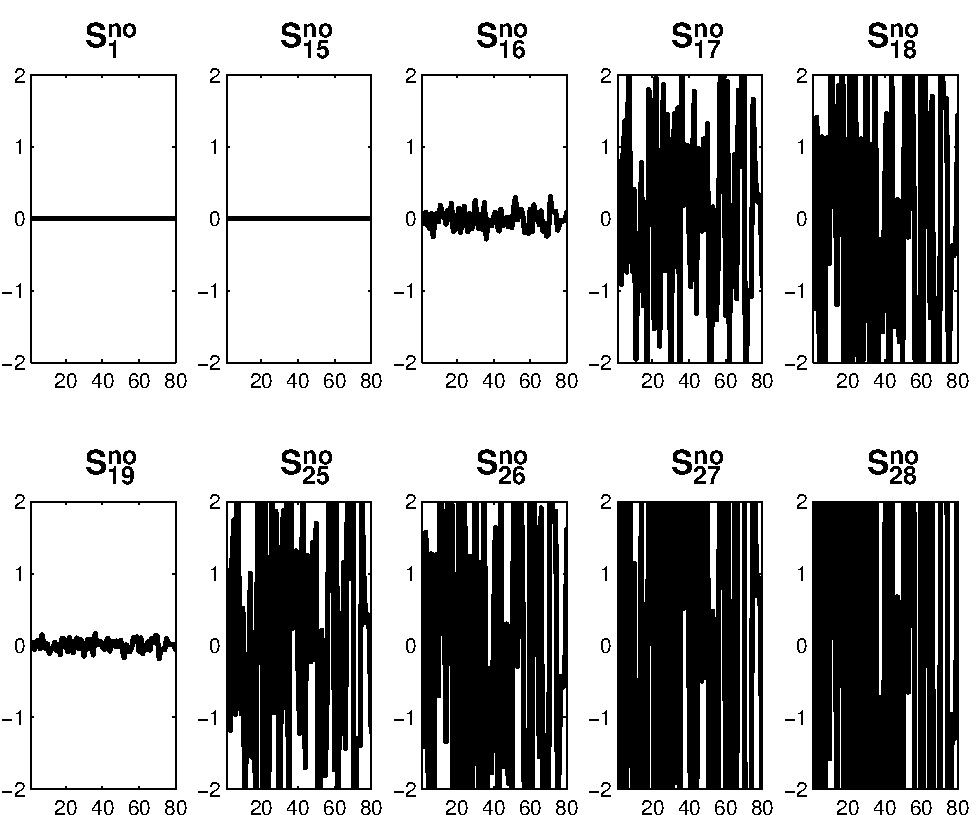
\includegraphics[width=.75\linewidth]{figures/run1/noise_parts} 
   
	\end{minipage}
	\begin{center}
		FIGURE: 
		The noise becomes visible at $s_17$, so $k_{noise} = 17$.
	\end{center} 
	\vspace{5mm}
	%%%%%%%%%%%%%%%%%%%%%%%%%%%%%%%%%%%%%%%%%%%%%%

	
	
	%%%%%%%%%%%%%%%%%%%%%%%%%%%%%%%%%%%%%%%%%%%%%%
	\vspace{5mm}
	\begin{minipage}[t]{0.5\textwidth}
	
		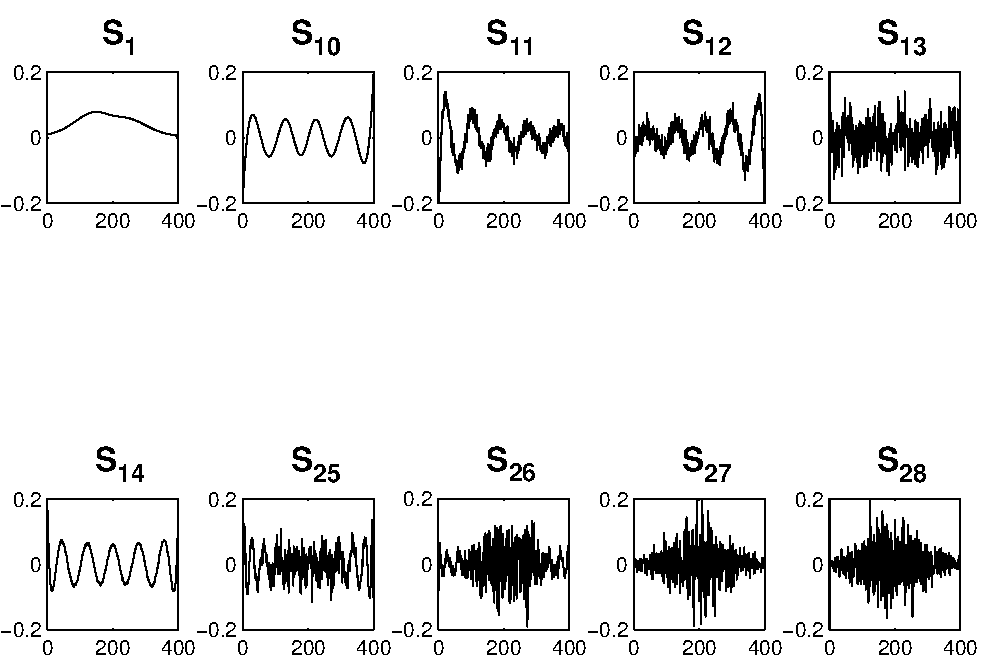
\includegraphics[width=.95\linewidth]{figures/run2/sk_plots} 
   
	\end{minipage}
	\begin{minipage}[t]{0.5\textwidth}
	
		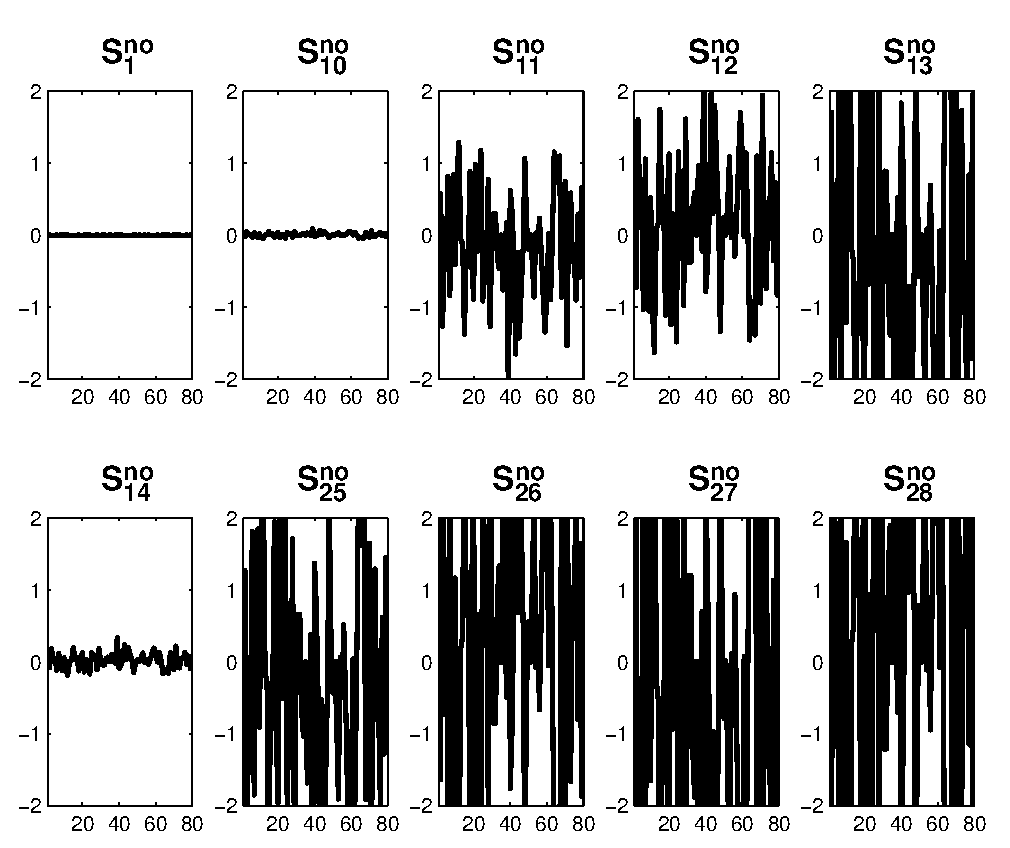
\includegraphics[width=.75\linewidth]{figures/run2/noise_parts} 
   
	\end{minipage}
	\begin{center}
		FIGURE: 
		Noise starts to become visible at the $s_{11}$ plot so $k_{noise}=11$
	\end{center} 
	\vspace{5mm}
	%%%%%%%%%%%%%%%%%%%%%%%%%%%%%%%%%%%%%%%%%%%%%%
	
	%%%%%%%%%%%%%%%%%%%%%%%%%%%%%%%%%%%%%%%%%%%%%%
	\vspace{5mm}
	\begin{minipage}[t]{0.5\textwidth}
	
		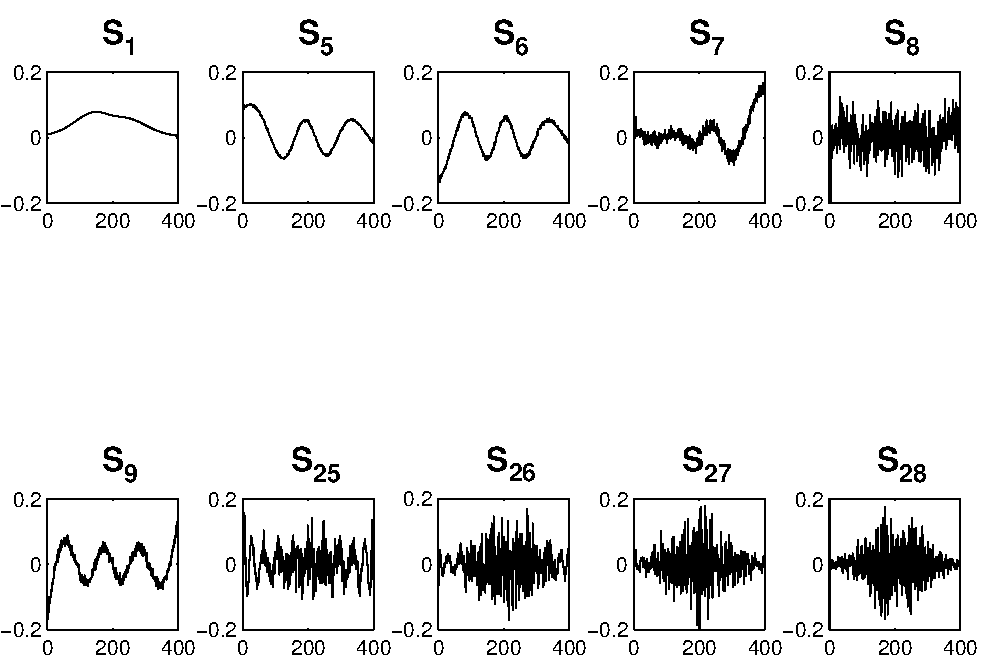
\includegraphics[width=.95\linewidth]{figures/run3/sk_plots} 
   
	\end{minipage}
	\begin{minipage}[t]{0.5\textwidth}
	
		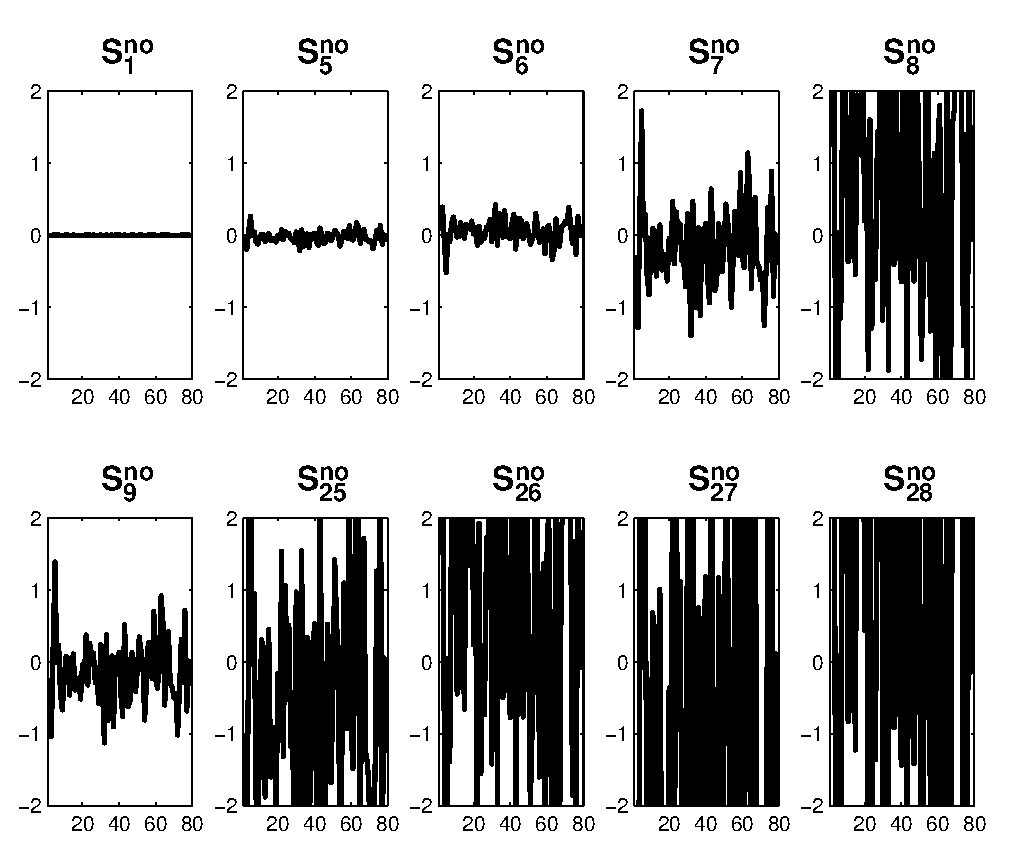
\includegraphics[width=.75\linewidth]{figures/run3/noise_parts} 
   
	\end{minipage}
	\begin{center}
		FIGURE: 
		Noise starts to become visible at the $s_{7}$ plot so $k_{noise}=7$
	\end{center} 
	\vspace{10mm}
	%%%%%%%%%%%%%%%%%%%%%%%%%%%%%%%%%%%%%%%%%%%%%%
	
	%%%%%%%%%%%%%%%%%%%%%%%%%%%%%%%%%%%%%%%%%%%%%%
	\vspace{10mm}
	\begin{minipage}[t]{0.5\textwidth}
	
		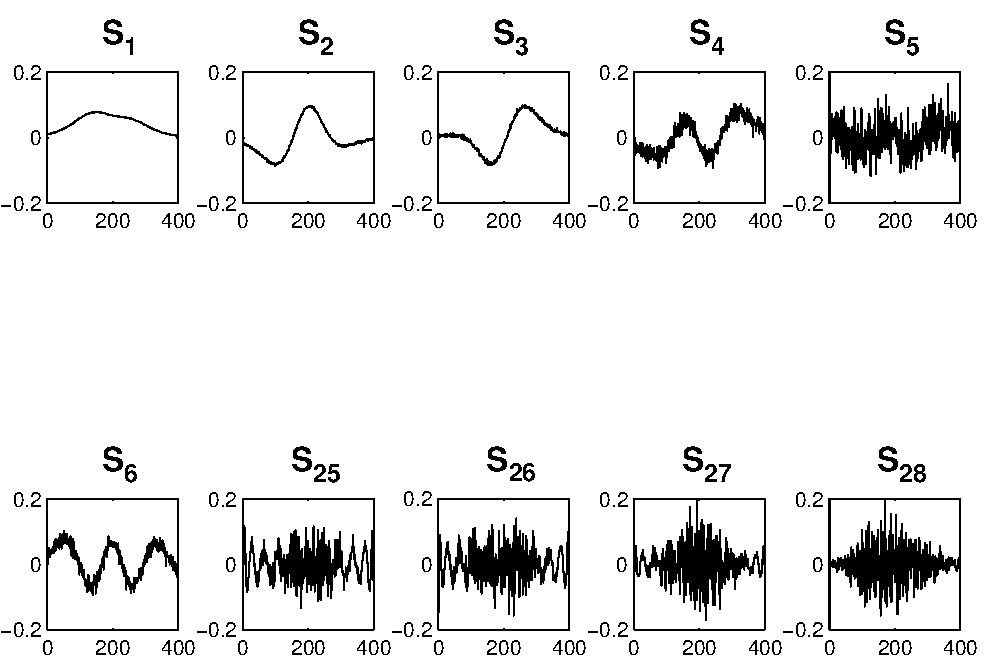
\includegraphics[width=.95\linewidth]{figures/run4/sk_plots} 
   
	\end{minipage}
	\begin{minipage}[t]{0.5\textwidth}
	
		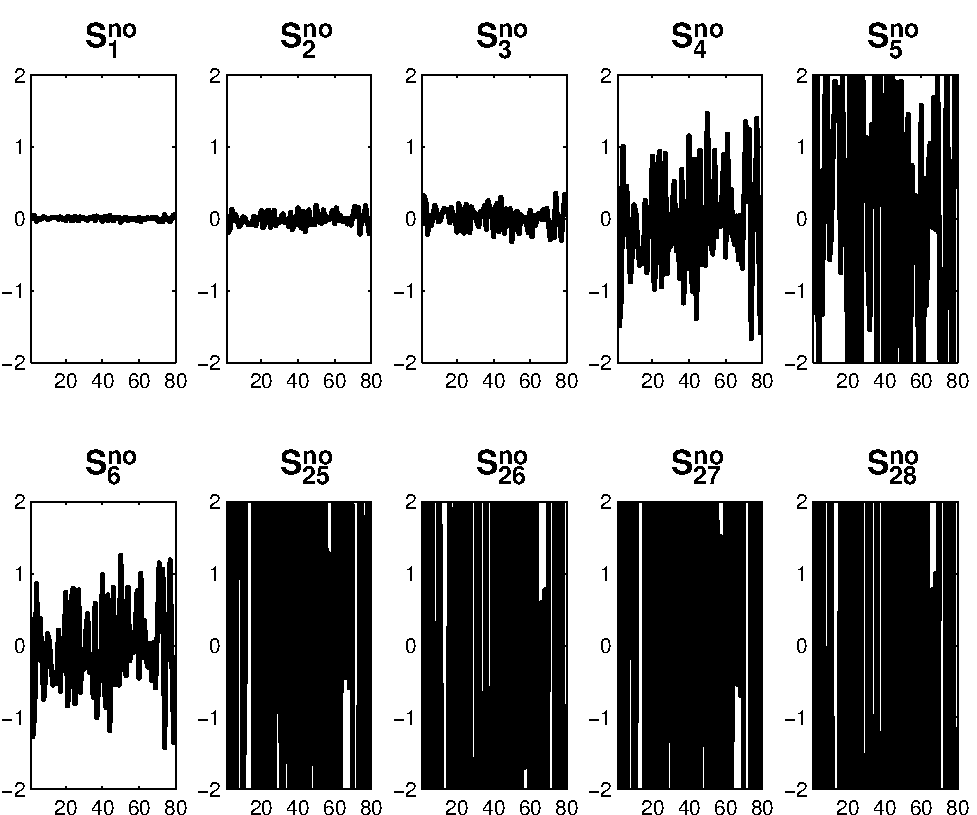
\includegraphics[width=.75\linewidth]{figures/run4/noise_parts} 
   
	\end{minipage}
	\begin{center}
		FIGURE: 
		Noise starts to become visible at the $s_{4}$ plot so $k_{noise}=4$	\end{center} 
	\vspace{10mm}
	%%%%%%%%%%%%%%%%%%%%%%%%%%%%%%%%%%%%%%%%%%%%%%
	
	
	As we can see in the above plots, for larger values of $\delta_{noise}$, the
	noise is revealed at earlier iterations. We also see that once the noise enters
	the $s_k$ vectors for the first time, the plots of $s_k$(left) appear to have 
	reduced amount of noise in the immediately following iteration but this 
	noise never leaves the vectors. This observation can also be seen on the
	plots of $s_{k}^{no}$(right).

\subsection{Finding $\bf k_{noise}$ using NCP} \indent \\
First we present the plot that we discussed during the presentation. This is the case where
$\delta_{noise} = 10^{-14}$  and the $\delta_{KS}=1.35$. Here, $\delta_{KS}$ is half of the
width of the Kolmogorov-Smirnov($KS$) test band.The corresponding cumulative periodogram is given below. 
On the left is the periodogram of the vectors $s_k$. On the right is their total deviation from 
the diagonal "white noise" diagonal line in blue and the percentage of indices lying outside of the KS test band.



%%%%%%%%%%%%%%%%%%%%%%%%%%%%%%%%%%%%%%%%%%%%%%
	\vspace{5mm}
	\begin{minipage}[t]{0.5\textwidth}
	
		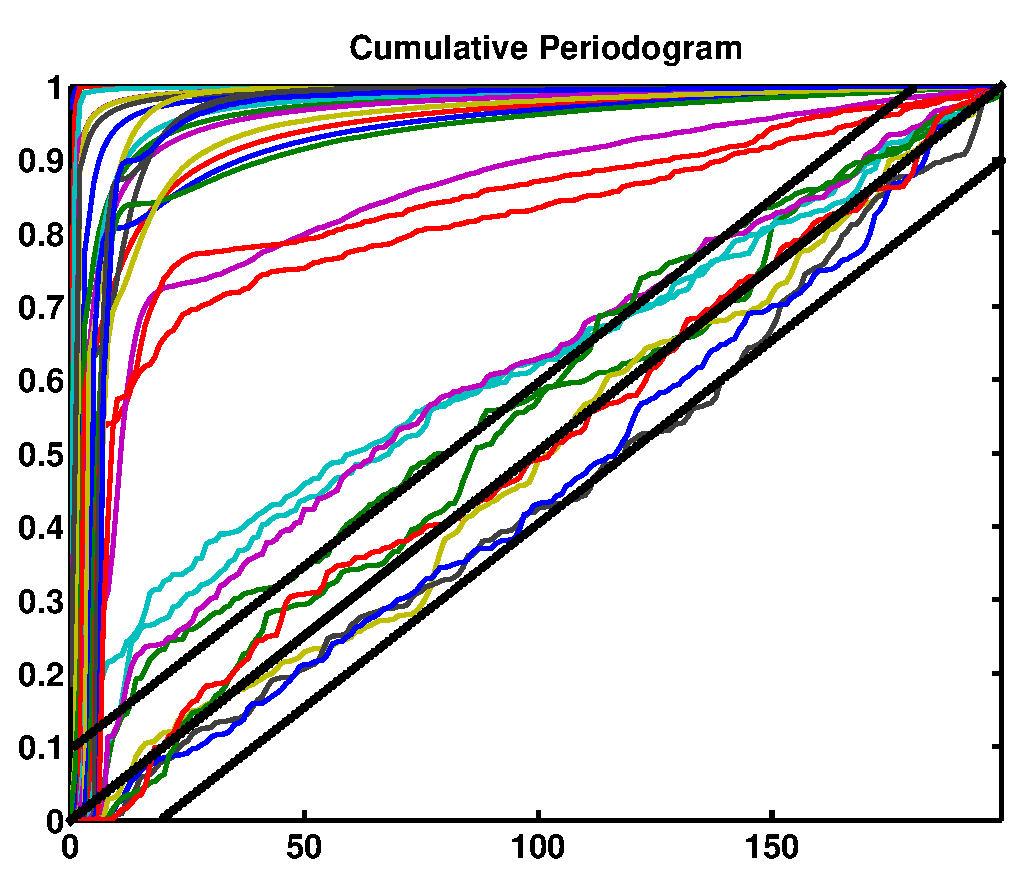
\includegraphics[width=.95\linewidth]{../presentation/figures/run1/cum_per} 
   
	\end{minipage}
	\begin{minipage}[t]{0.5\textwidth}
	
		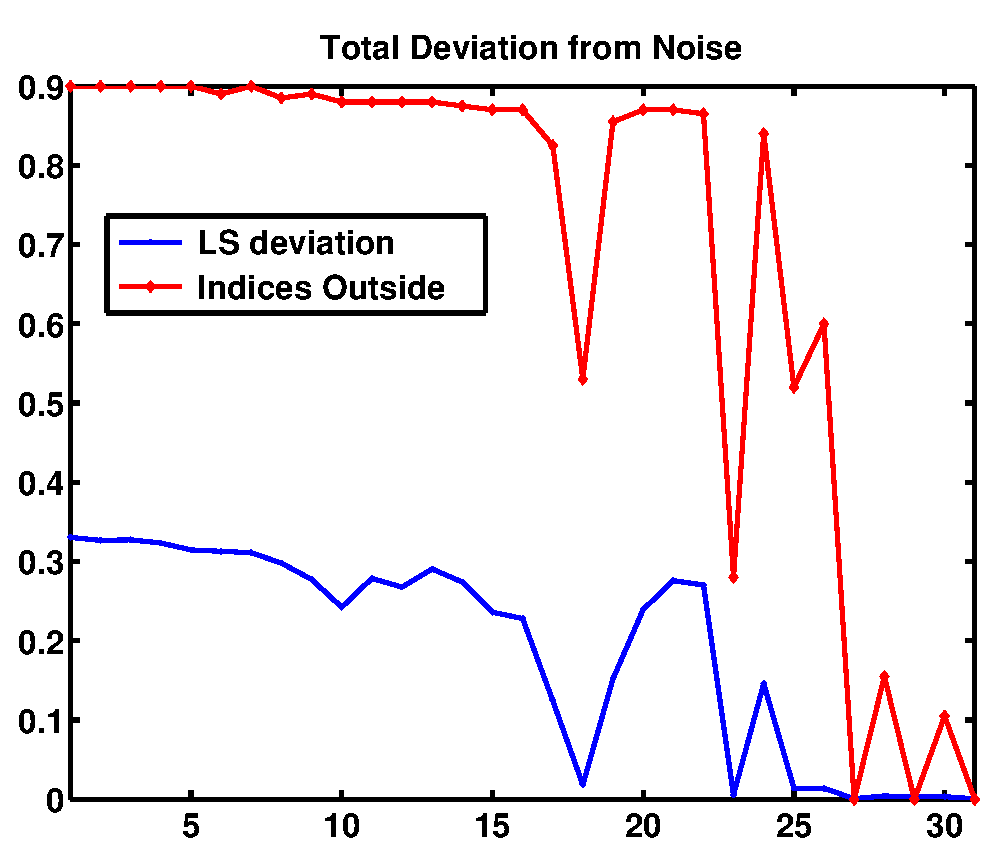
\includegraphics[width=.95\linewidth]{../presentation/figures/run1/total_deviation} 
   
	\end{minipage}
    \vspace{5mm}
	%%%%%%%%%%%%%%%%%%%%%%%%%%%%%%%%%%%%%%%%%%%%%%


As discussed in the presentation and can be see on the total deviation plot above, NCP
is determining that $k_{noise} = 27$. This value is in disagreement with the value determined
using KGB value of 17. Looking again at the total deviation plot, we can see that at iteration 17,
the total deviation is indeed a local minimum and then goes on to increase dramatically and then 
decrease again as it approaches iteration number 27. This is sort of to be expected given the
behavior of the $s_k$ vectors that was discussed above in which after the noise revealing
iteration, there is a decrease in visible noise and then eventually the vectors become more noisy. 
This is why if NCP does not consider this first local minimum to be $k_{noise}$, it won't
reach $k_{noise}$ until after noise is temporarily reduced from $s_k$ and then then increases
again.

This suggests that our criteria of what we call white noise may be too strict. If we widen our KS band
a bit we may be able to have NCP agree with KGB as to which iteration is the noise revealing iteration.
If we increase the $delta_{KS}$ value. After some experimentation we found that in order to get 
$k_{noise}$ from the first local minimum, the value of $\delta_{KS}$ must be at about 8.15.
We are not sure if making such modifications are allowed to be made with this test however.
Using $\delta_{KS}=8.15$ and $\delta_{noise}=10^{-14}$, we get the plots below:

%%%%%%%%%%%%%%%%%%%%%%%%%%%%%%%%%%%%%%%%%%%%%%
	\vspace{5mm}
	\begin{minipage}[t]{0.5\textwidth}
	
		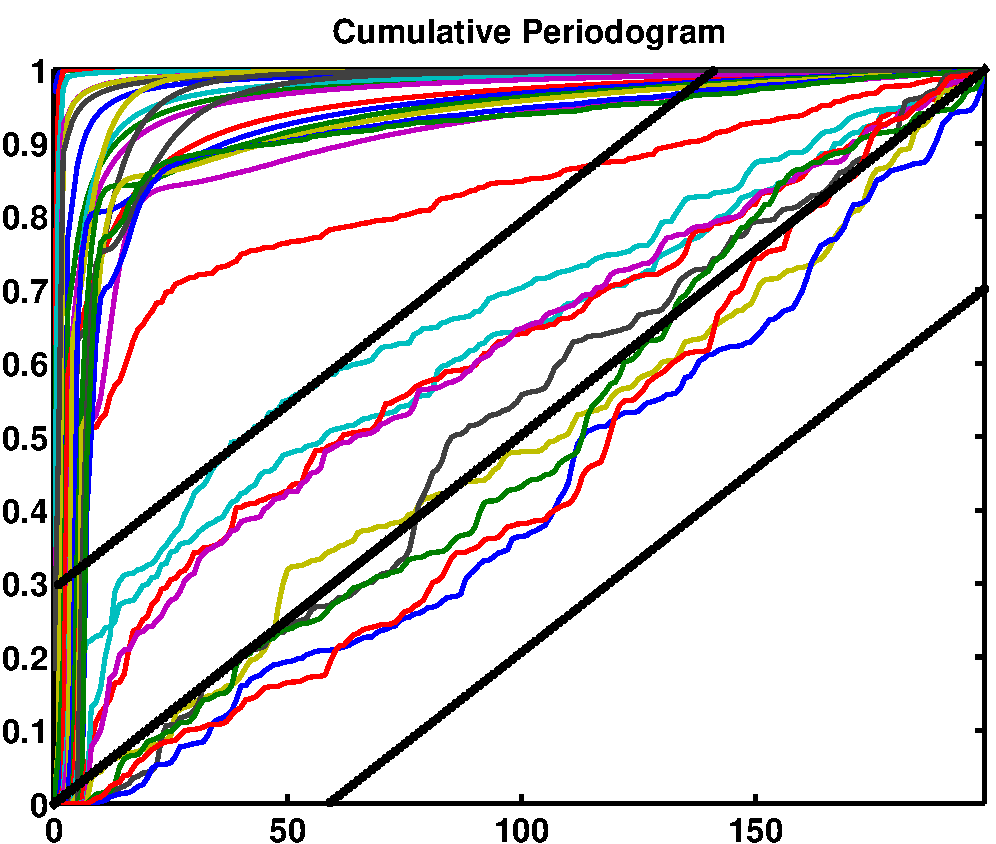
\includegraphics[width=.95\linewidth]{figures/run1/cum_per} 
   
	\end{minipage}
	\begin{minipage}[t]{0.5\textwidth}
	
		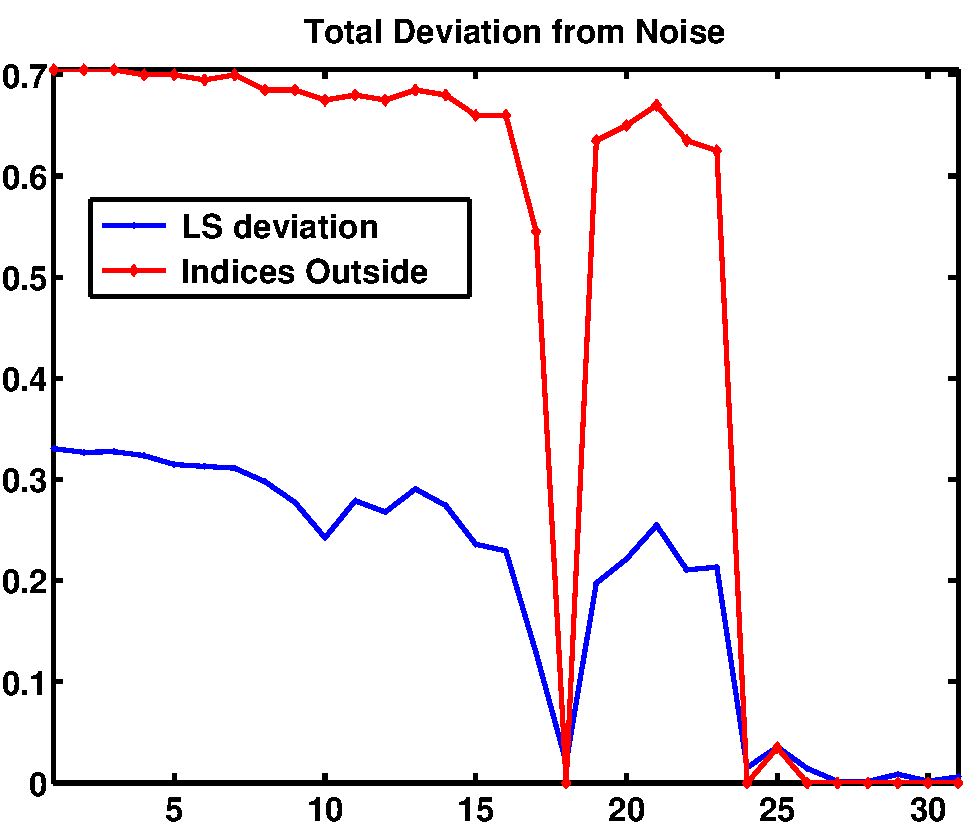
\includegraphics[width=.95\linewidth]{figures/run1/total_deviation} 
  
	\end{minipage}
{\centering $\delta_{noise}=10^{-14}$}
%%%%%%%%%%%%%%%%%%%%%%%%%%%%%%%%%%%%%%%%%%%%%%

%%%%%%%%%%%%%%%%%%%%%%%%%%%%%%%%%%%%%%%%%%%%%%
	\vspace{5mm}
	\begin{minipage}[t]{0.5\textwidth}
	
		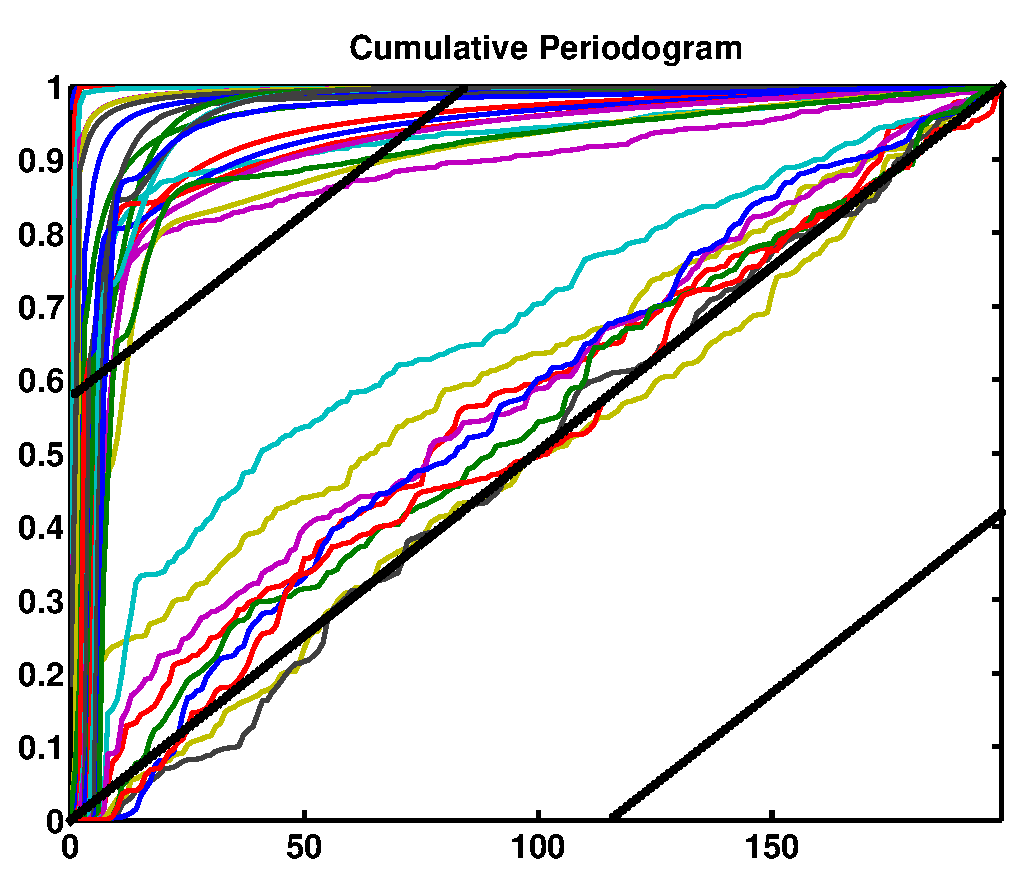
\includegraphics[width=.95\linewidth]{figures/run2/cum_per} 
   
	\end{minipage}
	\begin{minipage}[t]{0.5\textwidth}
	
		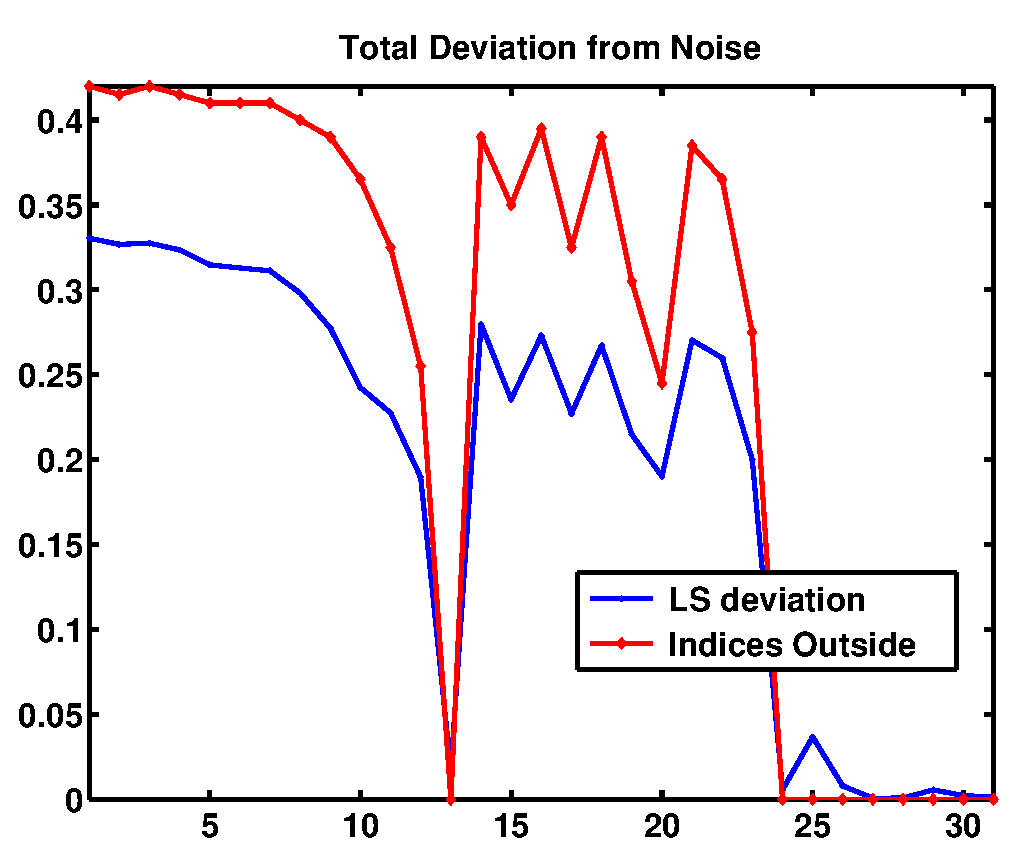
\includegraphics[width=.95\linewidth]{figures/run2/total_deviation} 
   
	\end{minipage}
	\vspace{5mm}
	{\centering $\delta_{noise}=10^{-8}$}
	%%%%%%%%%%%%%%%%%%%%%%%%%%%%%%%%%%%%%%%%%%%%%%
	
	%%%%%%%%%%%%%%%%%%%%%%%%%%%%%%%%%%%%%%%%%%%%%%
	\vspace{5mm}
	\begin{minipage}[t]{0.5\textwidth}
	
		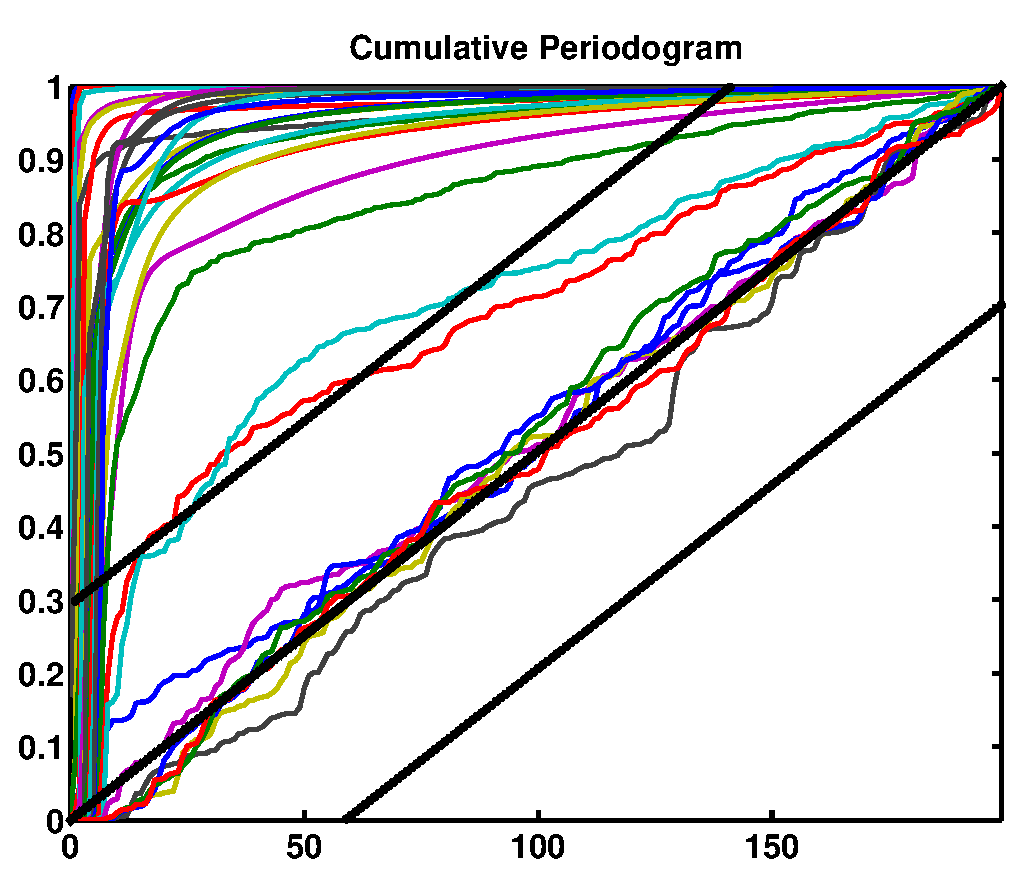
\includegraphics[width=.95\linewidth]{figures/run3/cum_per} 
   
	\end{minipage}
	\begin{minipage}[t]{0.5\textwidth}
	
		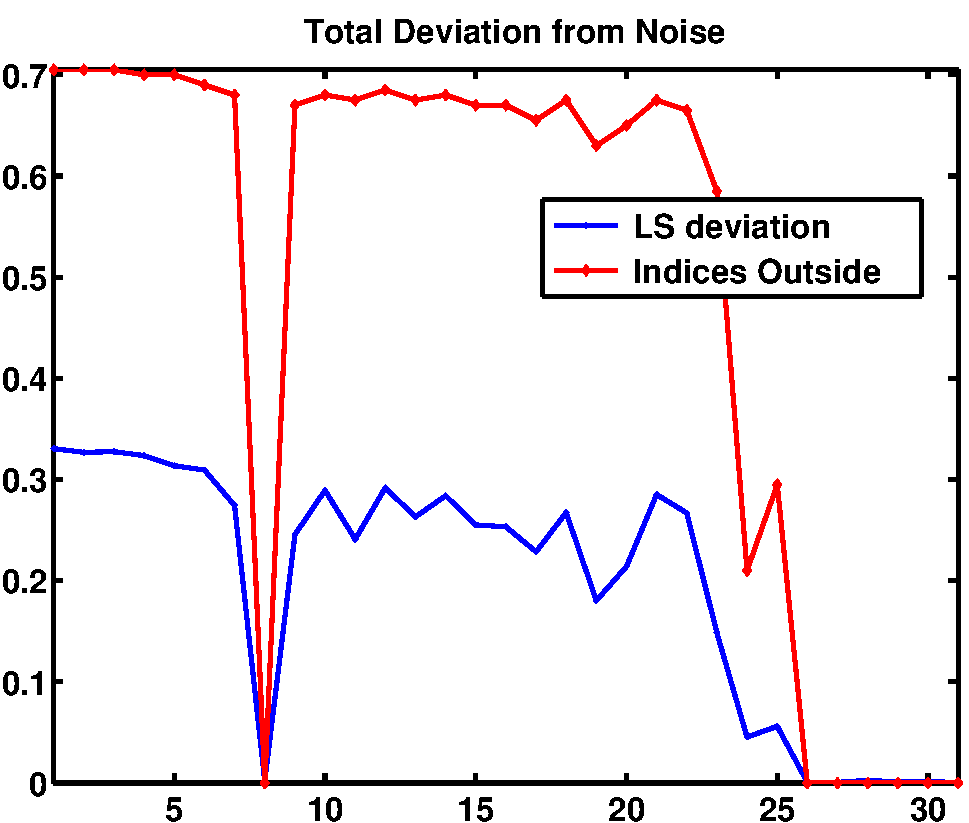
\includegraphics[width=.95\linewidth]{figures/run3/total_deviation} 
   
	\end{minipage}
	\vspace{5mm}
	{\centering $\delta_{noise}=10^{-4}$}
	%%%%%%%%%%%%%%%%%%%%%%%%%%%%%%%%%%%%%%%%%%%%%%
	
	%%%%%%%%%%%%%%%%%%%%%%%%%%%%%%%%%%%%%%%%%%%%%%
	\vspace{5mm}
	\begin{minipage}[t]{0.5\textwidth}
	
		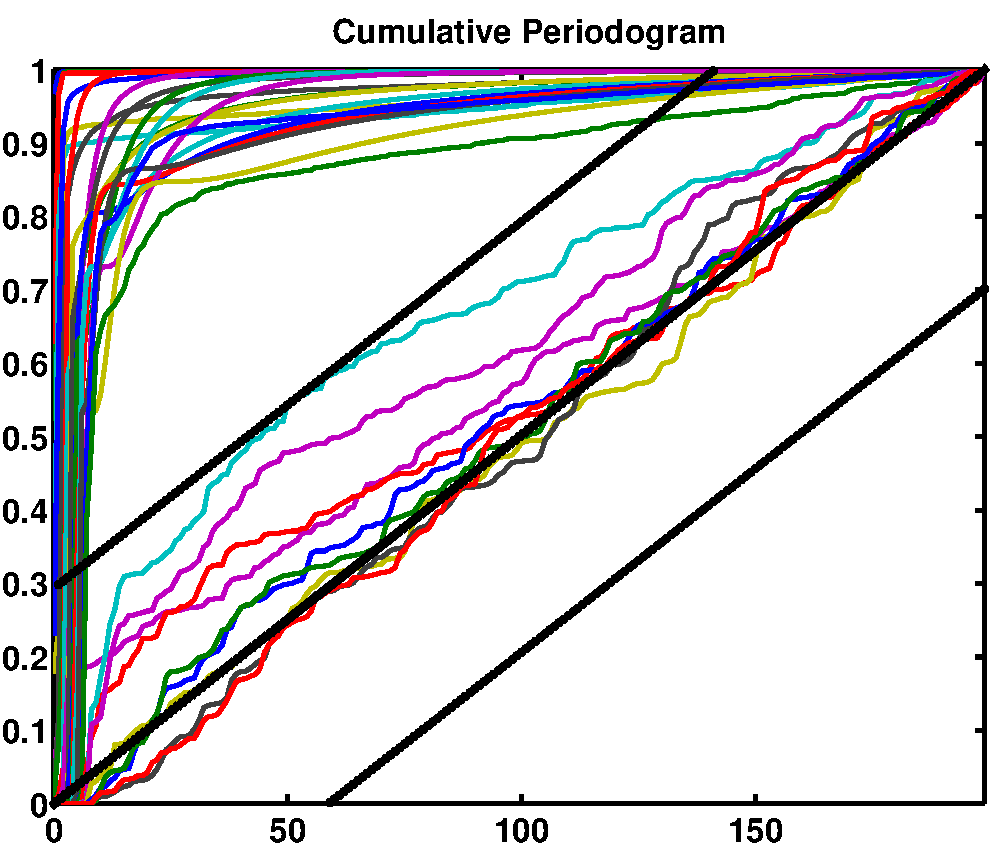
\includegraphics[width=.95\linewidth]{figures/run4/cum_per} 
   
	\end{minipage}
	\begin{minipage}[t]{0.5\textwidth}
	
		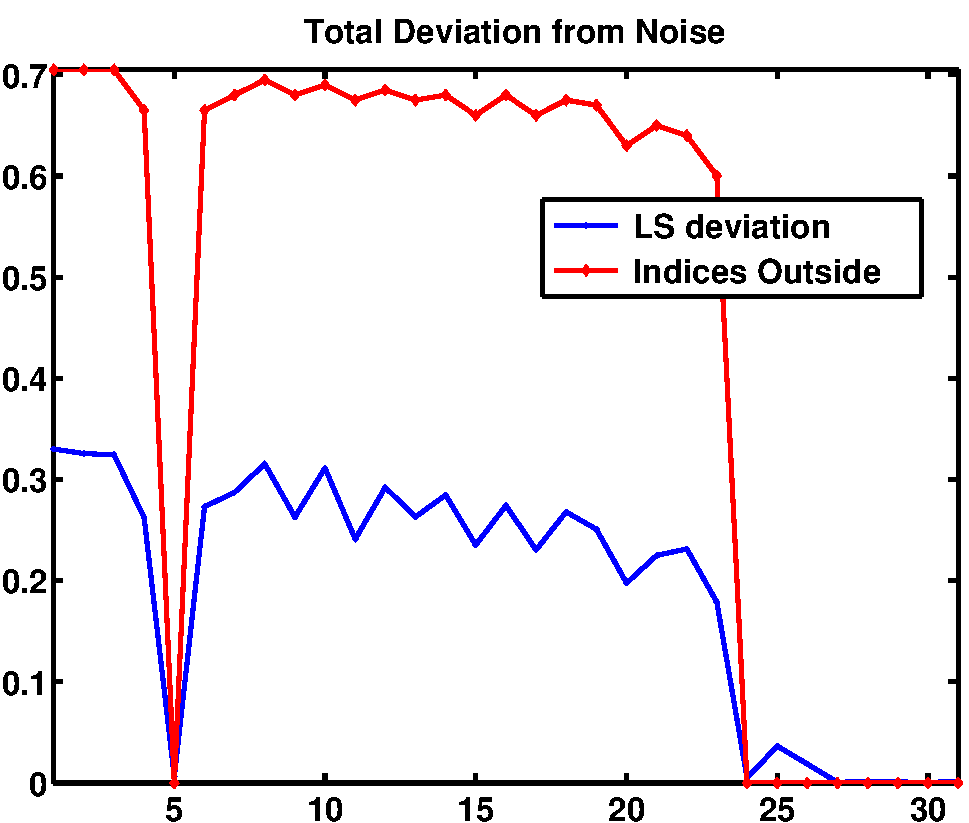
\includegraphics[width=.95\linewidth]{figures/run4/total_deviation} 
   
	\end{minipage}
		\vspace{5mm}
		{\centering $\delta_{noise}=10^{-2}$}
	%%%%%%%%%%%%%%%%%%%%%%%%%%%%%%%%%%%%%%%%%%%%%%
	
As we can see from the plots above, with the new value of $\delta_{KS}$, NCP finds $k_{noise}$
at the first dip as desired. One thing to note however is that in the code, the value of $k_noise$
was always one greater than the value found using GKB. In order to have the next vector be in the
KS band, we would need to make $\delta_{KS}$ much largr.
\end{document}  